%------------------------------------------------------------------------------
\section{Software Engineering for Economists}
%------------------------------------------------------------------------------

I teach students basic Software Engineering.

%------------------------------------------------------------------------------
\subsection{Course}
%------------------------------------------------------------------------------

\begin{boenumerate}
\item \textit{How would you rate the course overall?}
%------------------------------------------------------------------------------
%------------------------------------------------------------------------------
\begin{figure}[h!]\centering
\scalebox{0.5}{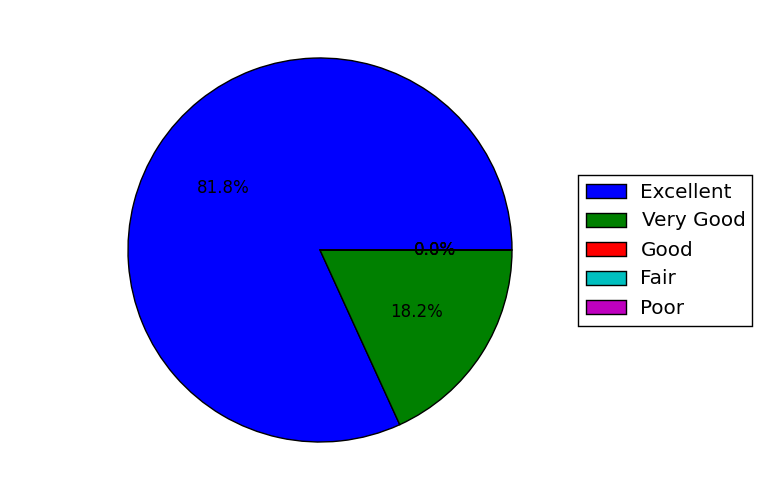
\includegraphics{../graphs/overall.png}}\hspace{0.75cm}
\begin{center}
\begin{minipage}[t]{0.85\columnwidth}\vspace{-0.75cm}
\item\scriptsize{\textbf{Notes:} Based on 11 student responses. }
\end{minipage}
\end{center}
\end{figure}
%------------------------------------------------------------------------------
%------------------------------------------------------------------------------
\item \textit{Which part of the University are you from?}

\begin{figure}[h!]\centering
\scalebox{0.5}{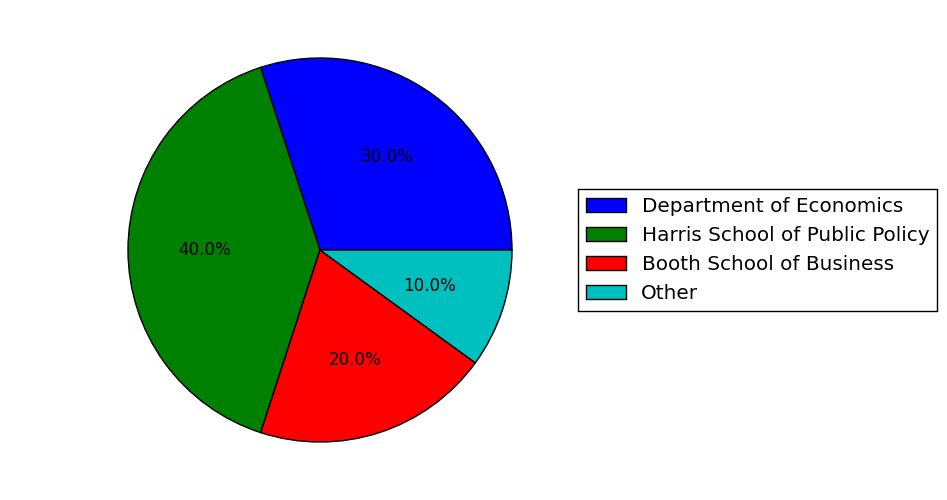
\includegraphics{../graphs/part_univ.png}}\hspace{0.75cm}
\begin{center}
\begin{minipage}[t]{0.85\columnwidth}\vspace{-0.75cm}
\item\scriptsize{\textbf{Notes:} Based on 10 student responses. }
\end{minipage}
\end{center}
\end{figure}
\newpage
%------------------------------------------------------------------------------
%------------------------------------------------------------------------------
\item \textit{Relative to your other classes, how useful was this course?}

\begin{figure}[h!]\centering
\scalebox{0.5}{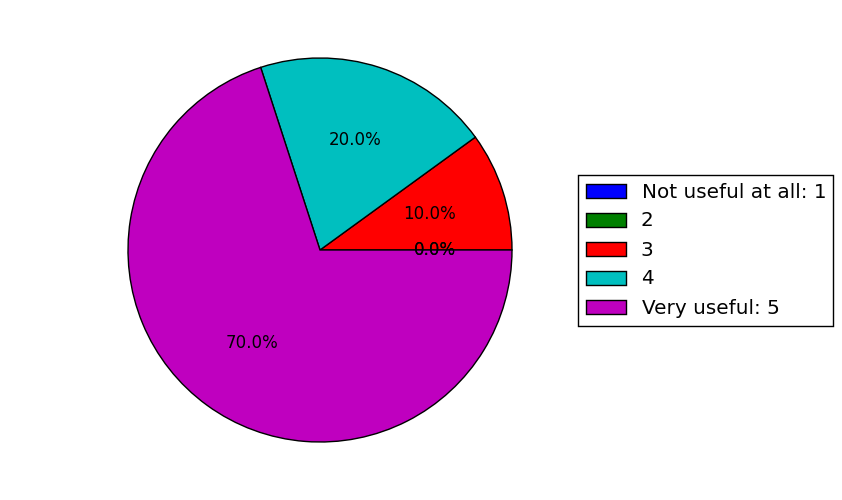
\includegraphics{../graphs/useful.png}}\hspace{0.75cm}
\begin{center}
\begin{minipage}[t]{0.85\columnwidth}\vspace{-0.75cm}
\item\scriptsize{\textbf{Notes:} Based on 10 student responses. }
\end{minipage}
\end{center}
\end{figure}
%------------------------------------------------------------------------------
%------------------------------------------------------------------------------

\item \textit{How well did Philipp meet his goal ...}
\begin{itemize}
\item \textit{to be well organized?}

\begin{figure}[h!]\centering
\scalebox{0.5}{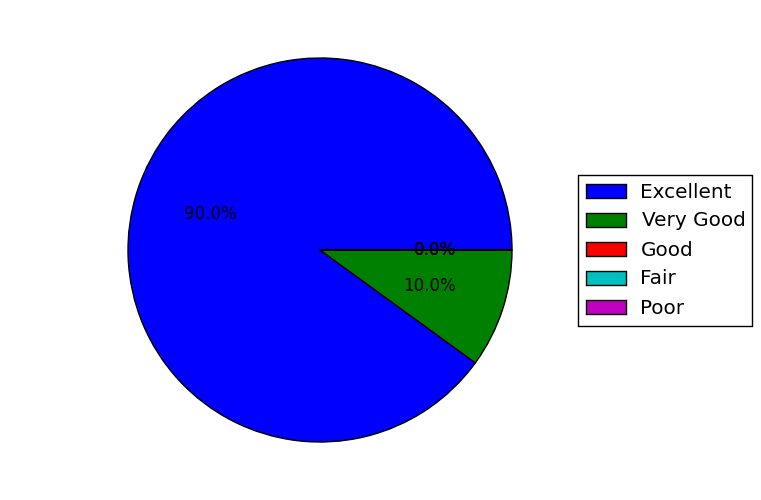
\includegraphics{../graphs/organized.png}}\hspace{0.75cm}
\begin{center}
\begin{minipage}[t]{0.85\columnwidth}\vspace{-0.75cm}
\item\scriptsize{\textbf{Notes:} Based on 10 student responses. }
\end{minipage}
\end{center}
\end{figure}

%------------------------------------------------------------------------------
%------------------------------------------------------------------------------

\item \textit{to present the material at the right speed?}

\begin{figure}[h!]\centering
\scalebox{0.5}{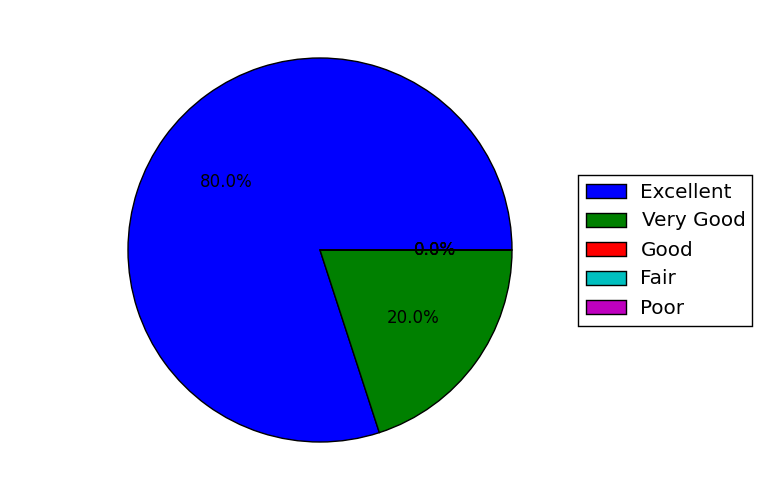
\includegraphics{../graphs/speed.png}}\hspace{0.75cm}
\begin{center}
\begin{minipage}[t]{0.85\columnwidth}\vspace{-0.75cm}
\item\scriptsize{\textbf{Notes:} Based on 10 student responses. }
\end{minipage}
\end{center}
\end{figure}

%------------------------------------------------------------------------------
%------------------------------------------------------------------------------

\item \textit{to present the material clearly and understandable?}

\begin{figure}[h!]\centering
\scalebox{0.5}{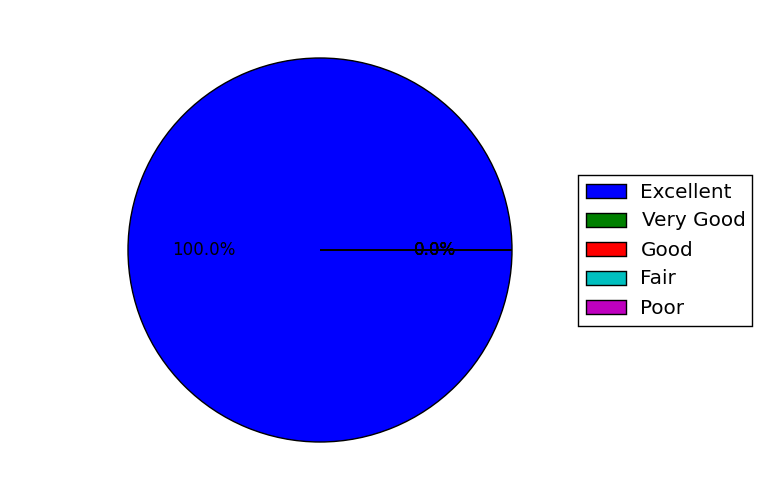
\includegraphics{../graphs/clearly.png}}\hspace{0.75cm}
\begin{center}
\begin{minipage}[t]{0.85\columnwidth}\vspace{-0.75cm}
\item\scriptsize{\textbf{Notes:} Based on 10 student responses. }
\end{minipage}
\end{center}
\end{figure}

%------------------------------------------------------------------------------
%------------------------------------------------------------------------------

\item \textit{to be accessible outside of class?}

\begin{figure}[h!]\centering
\scalebox{0.5}{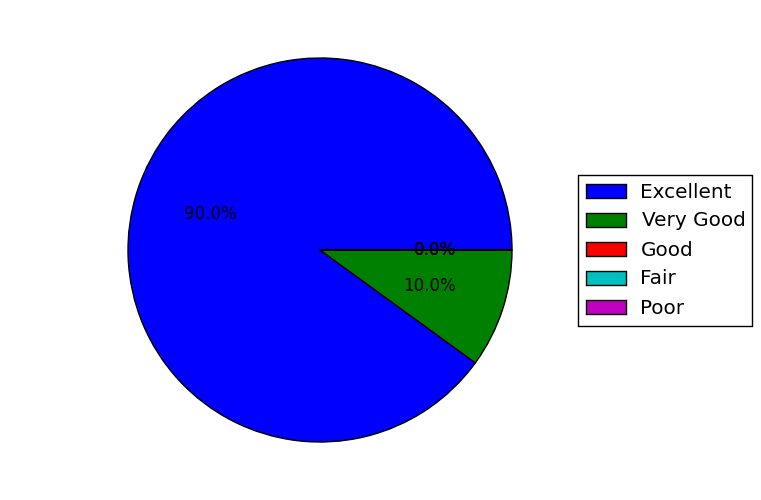
\includegraphics{../graphs/access.png}}\hspace{0.75cm}
\begin{center}
\begin{minipage}[t]{0.85\columnwidth}\vspace{-0.75cm}
\item\scriptsize{\textbf{Notes:} Based on 10 student responses. }
\end{minipage}
\end{center}
\end{figure}







\end{itemize}\end{boenumerate}

